\documentclass[german,version-2020-11]{uzl-thesis}

\UzLThesisSetup{
  %
  Logo-Dateiname        = {uzl-thesis-logo-itcs.pdf},
  Verfasst              = {am}{Institut für Software Engineering und Programming Languages},
  %
  % The titles:
  %
  Titel auf Deutsch     = {
    Können semantische Ähnlichkeiten von Wörtern die Schlussfolgerungen des gesunden Menschenverstands verbessern?  Eine Fallstudie mit Prover E und SUMO.
  }, 
  Titel auf Englisch    = {
    Can semantic similarities of words enhance common sense reasoning?  A case study with prover E and SUMO.
  },
  %
  % Author and supervisor:
  % 
  Autor                 = {Julian Britz},
  Betreuerin            = {Prof. Dr. Diedrich Wolter},
  % 
  % Optional: Supporting persons and institutions. The text should be
  % in German, even for an English thesis.
  %
  Mit Unterstützung von = {Moritz Bayerkuhnlein},
  %
  Bachelorarbeit,
  Studiengang           = {Informatik},
  %
  % Date on which the thesis is turned in German, formatted the
  % traditional German way:
  %
  Datum                 = {06. Juli 2025},
  %
  % The English abstract. You must always provide abstracts in German
  % and in English. 
  %
  Abstract              = {
    Abstract.
  },
  Zusammenfassung       = {
    Zusammenfassung.
  },
  %
  Alphabetische Bibliographie,
  % Alternatively:
  % Numerische Bibliographie
}
%
\UzLStyle{alegrya modern design}
%%%%%%%%
%
% Now, include the package you need here using \usepackage. 
%
% However, many standard packages are already loaded by the class:
%
% amsmath, amssymb, amsthm, babel, biblatex, csquotes, etoolbox,
% filecontents, fontspec, geometry, hyperref, tikz (with libraries
% arrows.meta, positioning and shapes), varioref, url 
%
% Indeed, in many cases you will not need any extra packages.
%
%%%%%%%





\begin{document}

%
% The title page and table of contents will be inserted automatically
% here. 
%


\chapter{Einleitung}
% In a German thesis write: \chapter{Einleitung}
  \begin{itemize}
    \item Bedeutung der logischen Schlussfolgerung im Bereich KI und der natürlichen Sprachverarbeitung
    \item Typische Ansätze
    \item Potenzial von semantischen Informationen zur Verbesserung der Auswahl von Axiomen
    \item Beschreibung von E als ein effektiver Theorembeweiser für die Aussagenlogik
    \item Adimen-SUMO als komplexe Wissensbasis für die Simulation und Bewertung von Schlussfolgerungsstrategien
    \item Ziel und Beitrag der Arbeit
  \end{itemize}
\chapter{Verwandte Arbeit}
\begin{itemize}
  \item ALR12. ´Alvez, Javier, Paqui Lucio and German Rigau: Adimen-SUMO:
  Reengineering an Ontology for First-Order Reasoning. Int. J. Semantic
  Web Inf. Syst., 8(4):80–116, 2012.
  \item Syntaktische Selektionsstrategien:
  \begin{itemize}
    \item HV11. Hoder, Krystof and Andrei Voronkov: Sine Qua Non for
    Large Theory Reasoning. In Bjørner, Nikolaj S. and Viorica
    Sofronie-Stokkermans (editors): Automated Deduction - CADE-
    23 - 23rd International Conference on Automated Deduction, Wroclaw,
    Poland, July 31 - August 5, 2011. Proceedings, volume 6803 of Lecture
    Notes in Computer Science, pages 299–314. Springer, 2011.
    \item Meng, Jia and Lawrence C. Paulson: Lightweight relevance filter-
    ing for machine-generated resolution problems. J. Appl. Log., 7(1):41–
    57, 2009.
    \item Roederer, Alex, Yury Puzis and Geoff Sutcliffe: Divvy: An
    ATP Meta-system Based on Axiom Relevance Ordering. In Schmidt,
    Renate A. (editor): Automated Deduction - CADE-22, 22nd Interna-
    tional Conference on Automated Deduction, Montreal, Canada, August
    2-7, 2009. Proceedings, volume 5663 of Lecture Notes in Computer Sci-
    ence, pages 157–162. Springer, 2009.
  \end{itemize}
  \item SInE: Roederer, Alex, Yury Puzis and Geoff Sutcliffe: Divvy: An
  ATP Meta-system Based on Axiom Relevance Ordering. In Schmidt,
  Renate A. (editor): Automated Deduction - CADE-22, 22nd Interna-
  tional Conference on Automated Deduction, Montreal, Canada, August
  2-7, 2009. Proceedings, volume 5663 of Lecture Notes in Computer Sci-
  ence, pages 157–162. Springer, 2009.
  \item Semantisch: Sutcliffe, Geoff and Yury Puzis: SRASS - A Semantic Relevance
  Axiom Selection System. In Pfenning, Frank (editor): Automated
  Deduction - CADE-21, 21st International Conference on Automated
  Deduction, Bremen, Germany, July 17-20, 2007, Proceedings, volume
  4603 of Lecture Notes in Computer Science, pages 295–310. Springer,
  2007.
\end{itemize}
%
\chapter{Behauptung}
Die semantische Nähe von Wörtern kann das Commen Sense Reasoning unterstützen.\\
Wieso? Grobe Beschreibung. Wie ist eine Grammatik strukturiert? Wie ist der Zusammenhang zwischen Logik und natürlicher Sprache? \\
Proover berücksichtigt nur die Signaturen und bringt solche in Verbindung, die in einer logischen Kette sind. \\
Wenn nun aber ein Begriff in dieser Kette nicht vorkommt, aber für den Beweis relevant ist, dann fehlt dies. \\

the semantic structure of ontologies often mirrors descriptions and categorizations found in natural language.

Ontologies might integrate or be constructed using existing language resources such as thesauri, taxonomies, or lexical databases (e.g., WordNet), which are themselves typically developed from natural language data.

Shared Semantic Goals:

Both natural language and ontologies aim to represent and convey meaning. While the methods and structures differ, they both operate within the realm of semantics—understanding and relating concepts and entities.

Complementary Roles:

Natural language is often the starting point for building ontologies, helping to identify and articulate the necessary concepts and properties. Ontologies, in turn, can support natural language processing by providing a structured, semantic backbone for interpreting text.

"The integration of natural language semantic similarity measures into the axiom selection process of automated theorem provers significantly enhances their performance in commonsense reasoning tasks, bridging the gap between human-like understanding and machine logic through improved alignment of logical axioms with linguistic context."

Behauptung: Logische Axiome tragen eine semantische Bedeutung, da sie einen Bezug zur realen Welt haben: Semantische Bedeutung: Auch wenn Axiome formal und symbolisch dargestellt werden, tragen sie eine semantische Bedeutung, da sie konzeptionelle Inhalte definieren, die mit bestimmten Bedeutungen in der realen Welt verbunden sind. Zum Beispiel könnte ein Axiom in einer Ontologie besagen, dass alle Menschen sterblich sind, was eine direkte semantische Verbindung zu unserem Wissen über die Realität hat.

Wie relevant ist die größe der Dimension und die max. sequenz-length
\chapter{Vorwissen}
  \section{Commen sense reasoning}
    \begin{itemize}
      \item Erklärung.
      \item Was ist das?
      \item Wofür braucht man es? Einsatzfelder
      \item Wie ist der aktuelle Stand?
      \item Herausforderungen
    \end{itemize}
  \section{Word Embeddings}
    \begin{itemize}
      \item Definition
      \item Erstellung
      \item Eigenschaften
      \item Anwendung
      \item Limitierung und Herausforderungen
    \end{itemize}
  \section{Grammatiken}
    \begin{itemize}
      \item Erklärung. Was sind Grammatiken und welche gibt es?
      \item Aufbau und Struktur
      \item Wofür benötigt man sie?
      \item SUMO
    \end{itemize}
  \section{Theorembeweiser}
    \begin{itemize}
      \item Erklärung. Was sind Theorembeweiser und welche gibt es?
      \item Funktionalität - wie werden Beweise gefunden - refutation
      \item Wofür braucht man sie?
      \item Grenzen und Herausforderungen
      \item Prover E
        \begin{itemize}
          \item Wie arbeitet E? Wie geht E vor?
          \item Satauto mode 
        \end{itemize}
    \end{itemize} 
\chapter{Selektionsstrategien}
  \begin{itemize}
    \item Syntaktisch 
    \item Semantisch
    \item Kombination - Union: wie übersetzt
  \end{itemize}
\chapter{Parallelen zwischen Sprachverarbeitung und Theorembeweisern}
\begin{itemize}
  \item Ziel: finde Worte/ Axiome, die zum Kontext passen, um eine gewisse Aussage zu erzielen
  \item Mehrdeutigkeiten werden mittels Resolution gelöst
  \item Both represent knowledge and meaning
  \item Ontologies like Adimen-SUMO capture entities, relationships, and properties formally, analogous to how natural language uses words, sentences, and grammar to convey meaning.
  \item Just as natural language has grammatical and syntactical rules, Adimen-SUMO is built upon logical syntax and rules. However, logical syntax is rigid and unambiguous, while natural language often allows for more flexibility and nuance
  \item Difference: While natural languages do have grammar and syntax, they are more flexible and context-dependent, allowing for ambiguity and multiple interpretations, unlike the rigid, unambiguous nature of formal logic.
  \item In natural language, much of the meaning is implicit, derived from context, tone, and prior knowledge. Logical systems make everything explicit, ensuring that every inference is clear and derivable from stated axioms
\end{itemize}
\chapter{Experimente}
  \begin{itemize}
    \item Whitebox Truth Test: wie werden diese erzeugt? \\ 
    \url{https://www.researchgate.net/publication/317230162_Automatic_White-Box_Testing_of_First-Order_Logic_Ontologies} \\ 
    Falsity tests created according to Adimen Sumo -> negate them to get falsity test -> Prover does refutation
    \clearpage
    \item Standard
    Self made results of Claudia Schon
    \begin{figure}[h!]
      \centering
      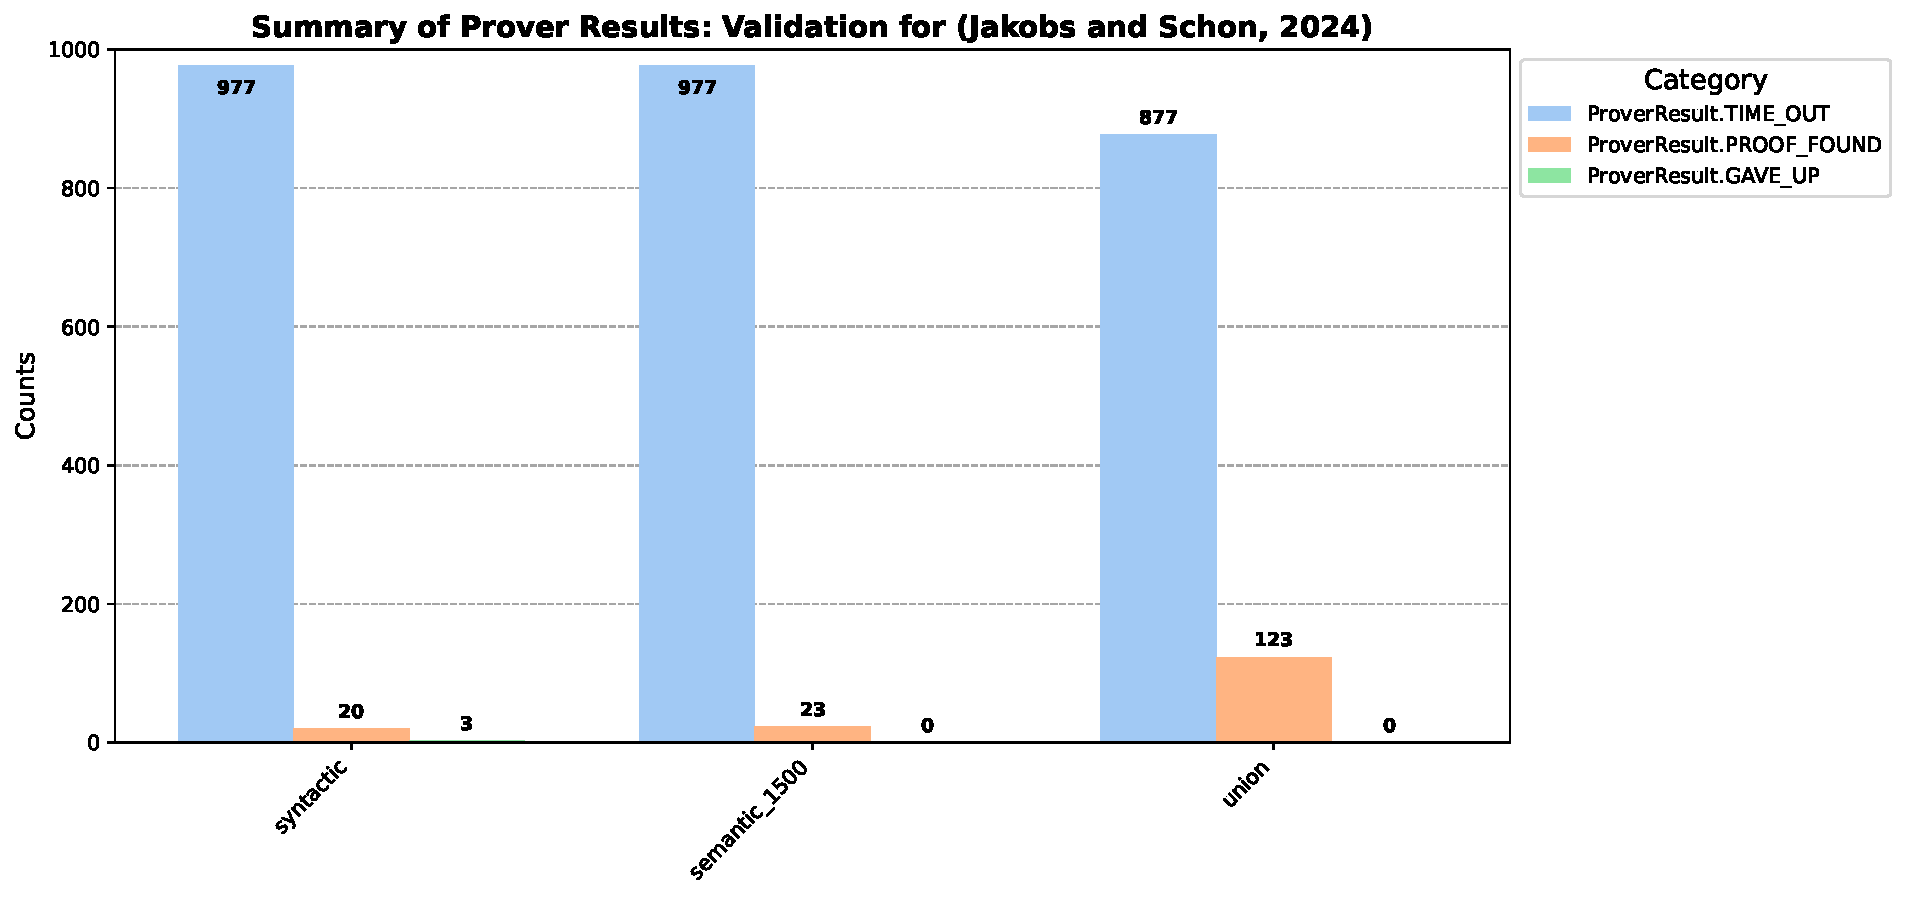
\includegraphics[width=\textwidth]{standard_mode_noAdded_output.pdf} % Add path to the PDF image
      \caption{Summary of Prover Results: Standard Mode}
      \label{fig:prover_results_standard}
    \end{figure}
    \clearpage
    \item Mean variable count
    Analyze the runs. Find that there are no clear statements that offer conclusions.
    \begin{figure}[h!]
      \centering
      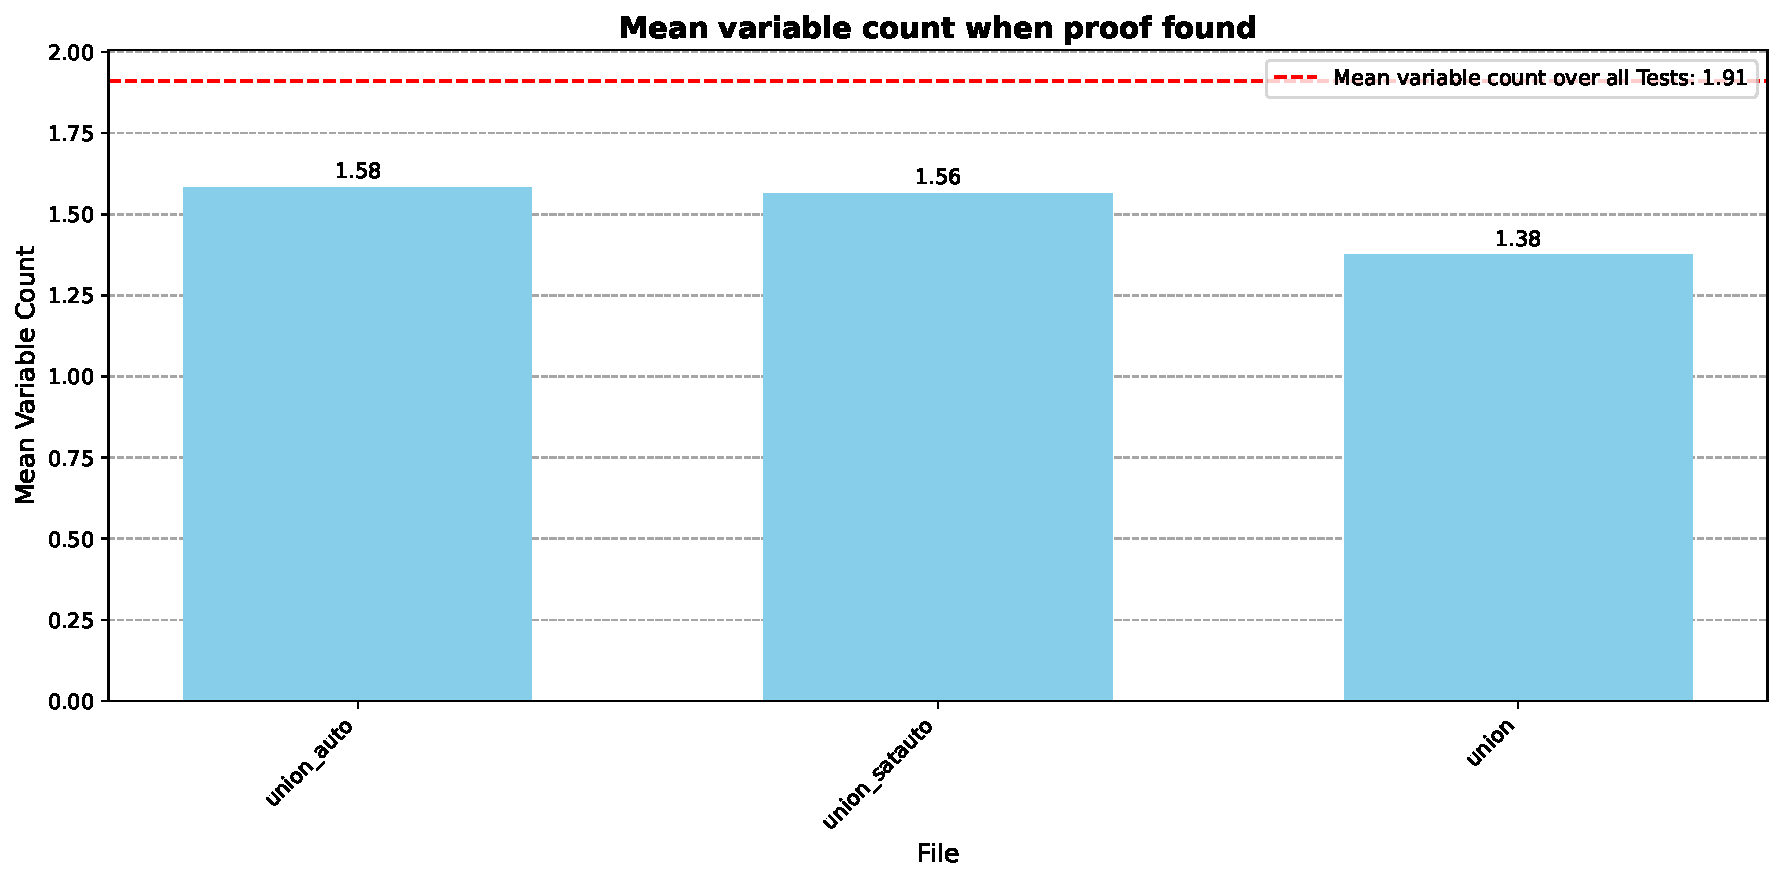
\includegraphics[width=\textwidth]{variable_count.pdf} % Add path to the PDF image
      \caption{Summary of Prover Results: Variable Count}
      \label{fig:prover_results_vampire}
    \end{figure}
    \clearpage
    \item Count signs
    \begin{figure}[h!]
      \centering
      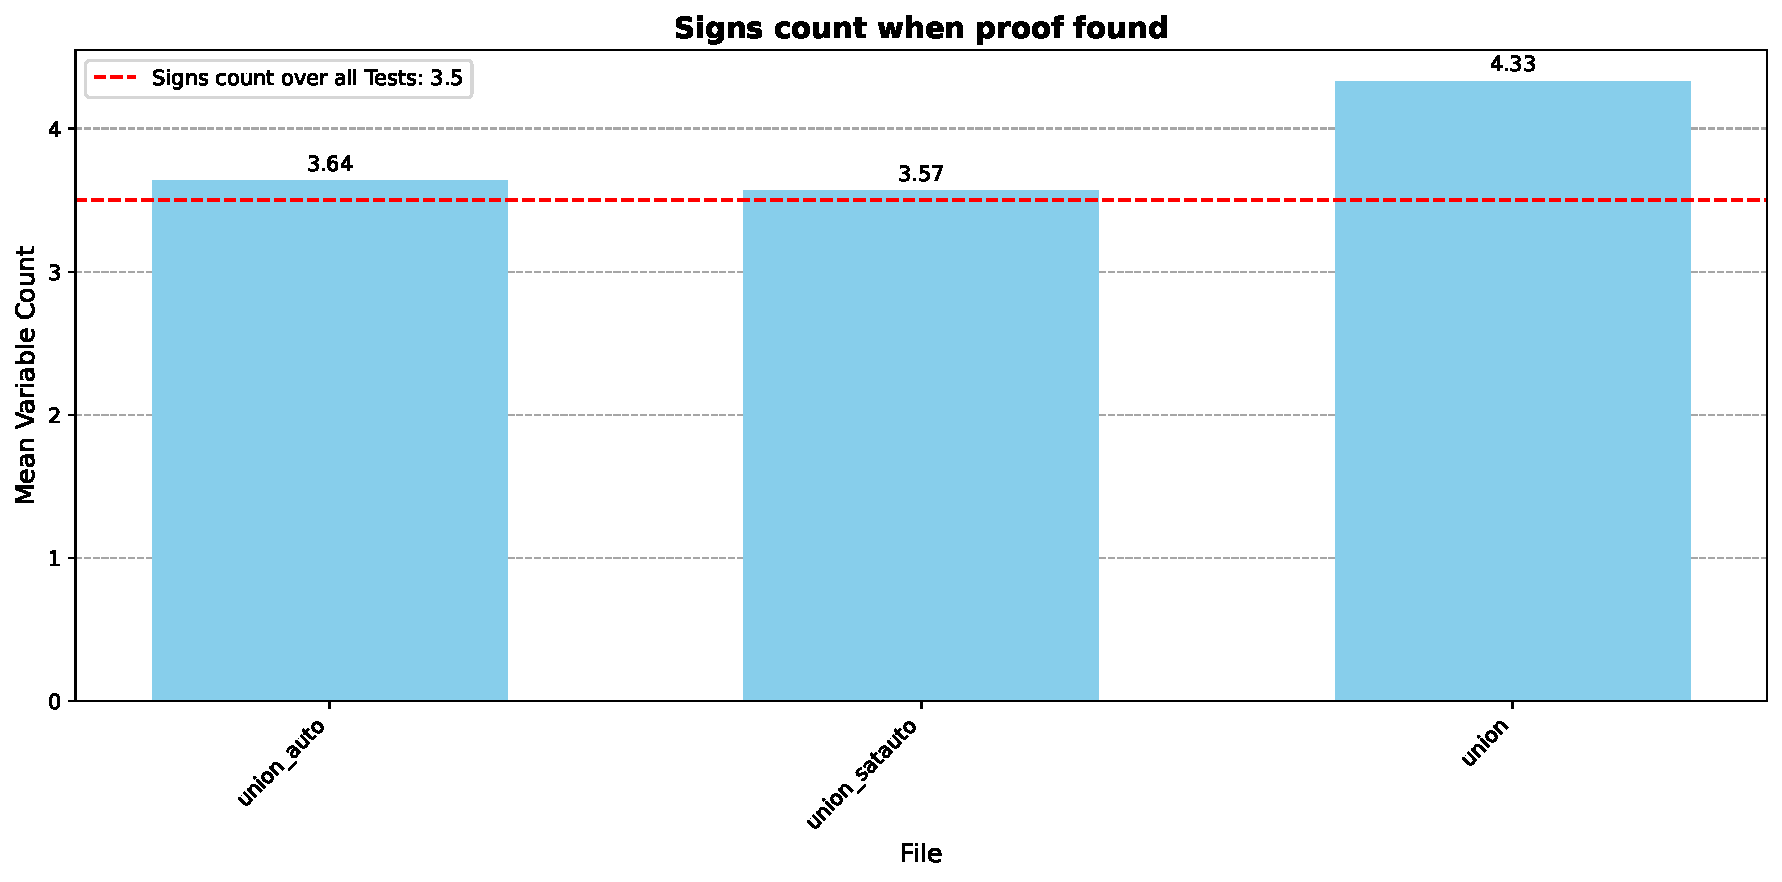
\includegraphics[width=\textwidth]{signs_count.pdf} % Add path to the PDF image
      \caption{Summary of Prover Results: Signs Count}
      \label{fig:prover_results_vampire}
    \end{figure}
    \clearpage
    \item Character Count
    \begin{figure}[h!]
      \centering
      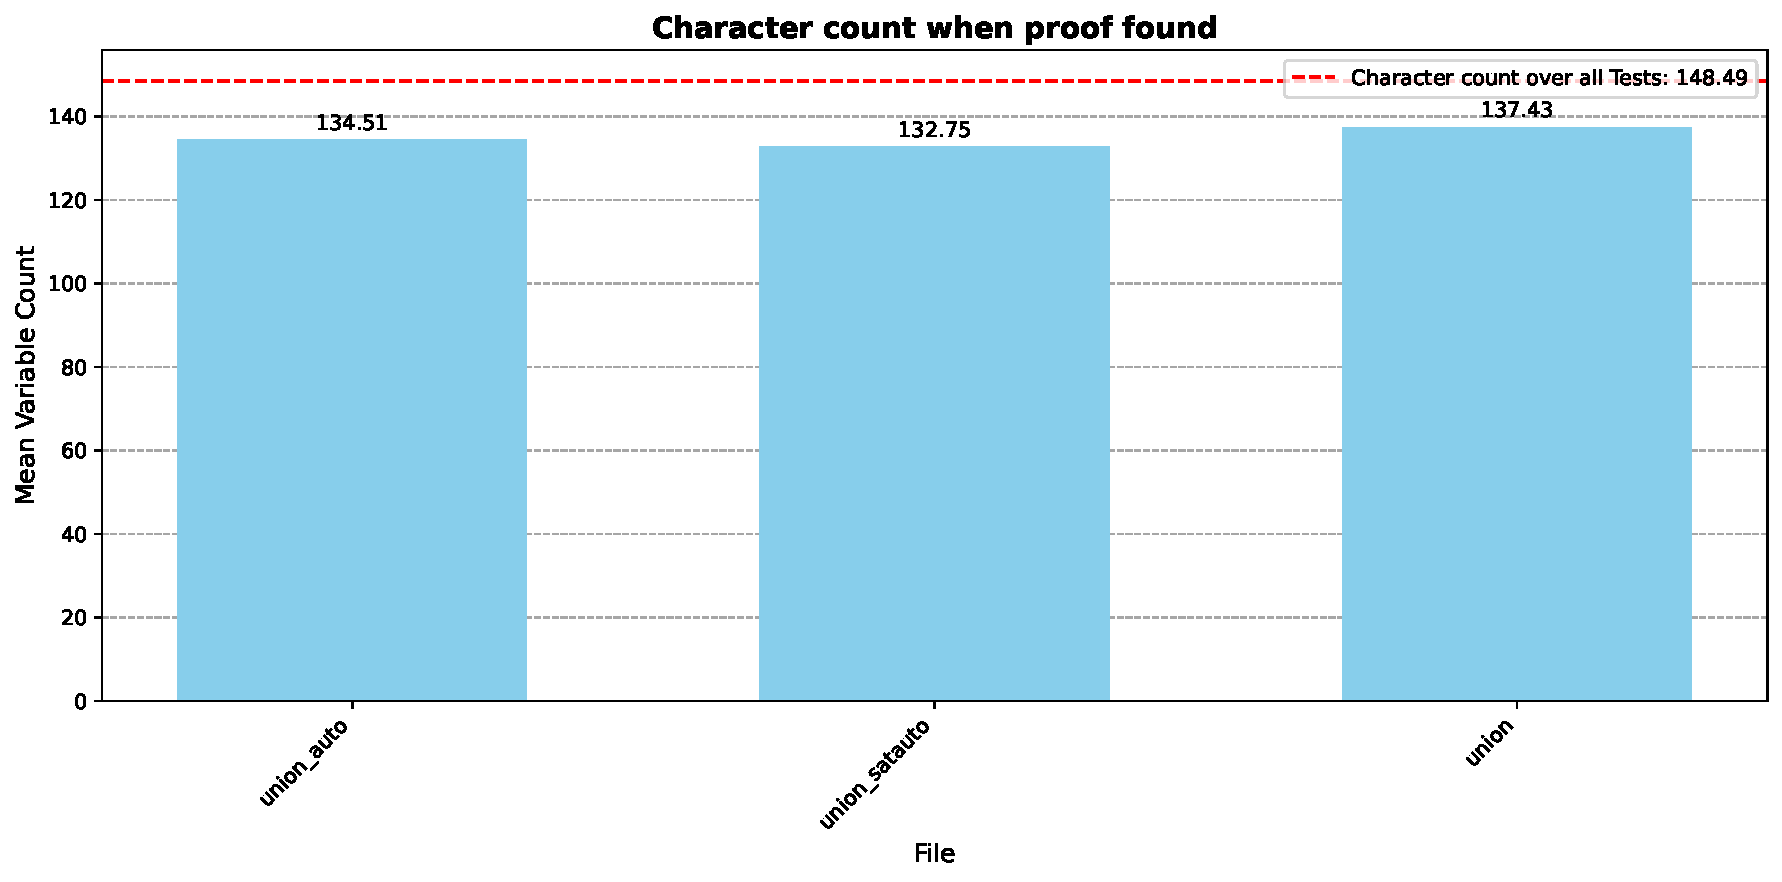
\includegraphics[width=\textwidth]{character_count.pdf} % Add path to the PDF image
      \caption{Summary of Prover Results: Character Count}
      \label{fig:prover_results_vampire}
    \end{figure}
    \clearpage
    \item Analyze Cosine Similarity
    \begin{figure}[h!]
      \centering
      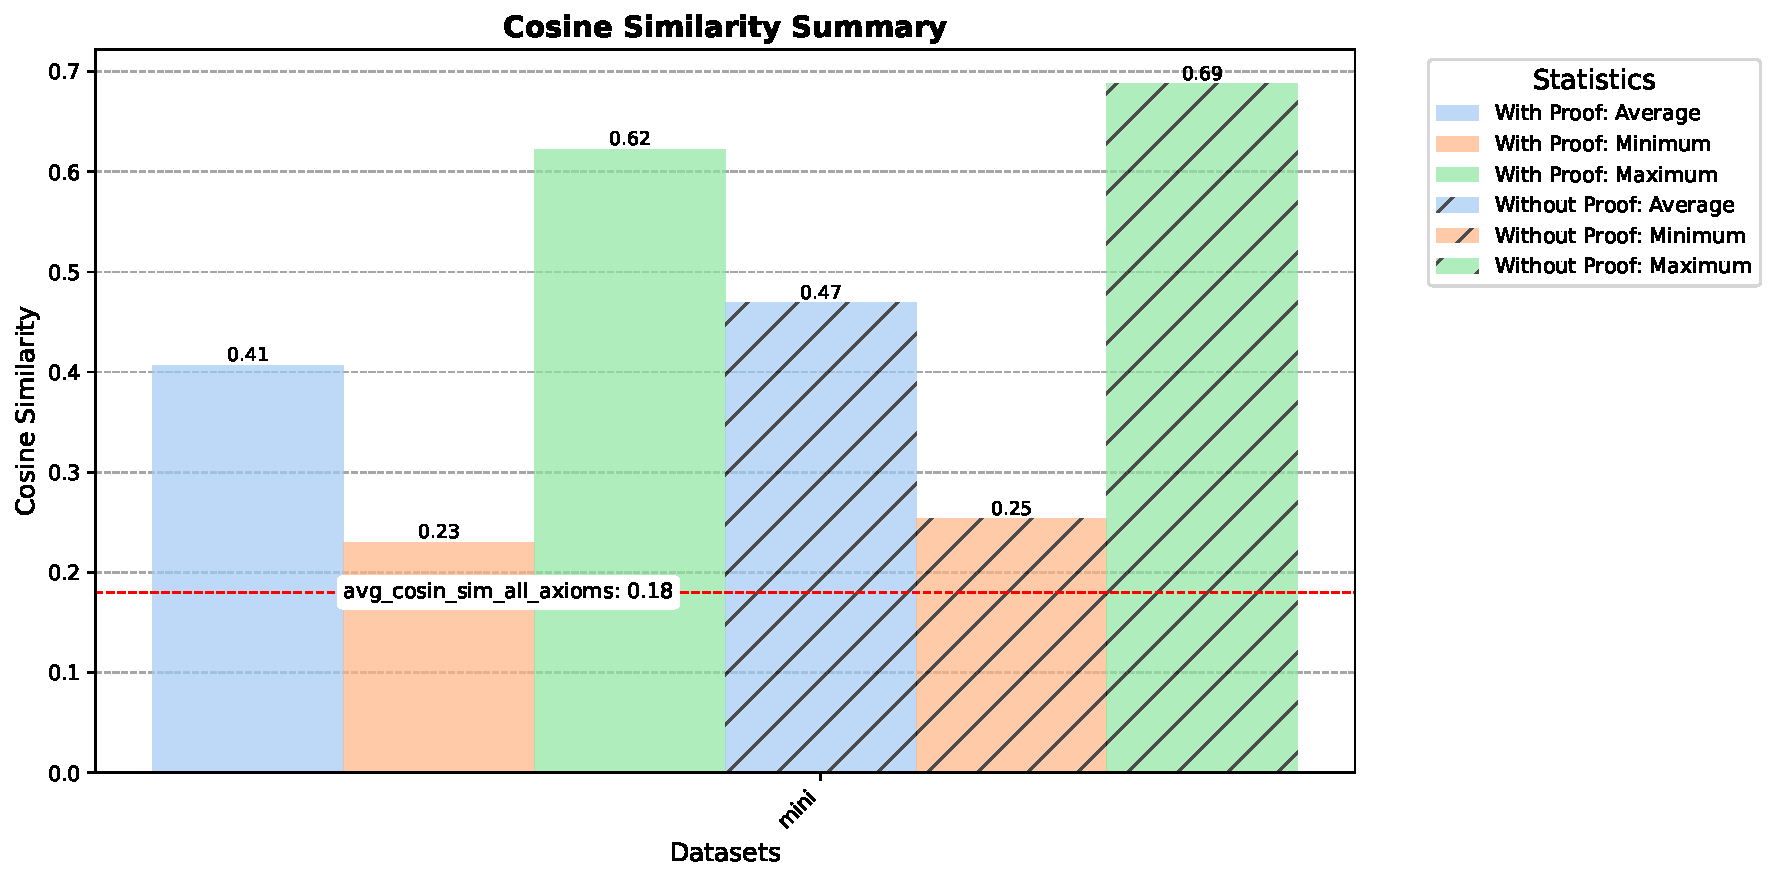
\includegraphics[width=\textwidth]{cosine_similarity_mini_noAdded_summary.pdf} % Add path to the PDF image
      \caption{Cosine No Added}
      \label{fig:prover_results_standard}
    \end{figure}
    Why Would Provable Conjectures Have Lower Axiom Similarity? This suggests that proving the conjecture involves bridging different concepts, rather than just refining a single closely related idea
    \clearpage
    \item Added Axiom
    \begin{figure}[h!]
      \centering
      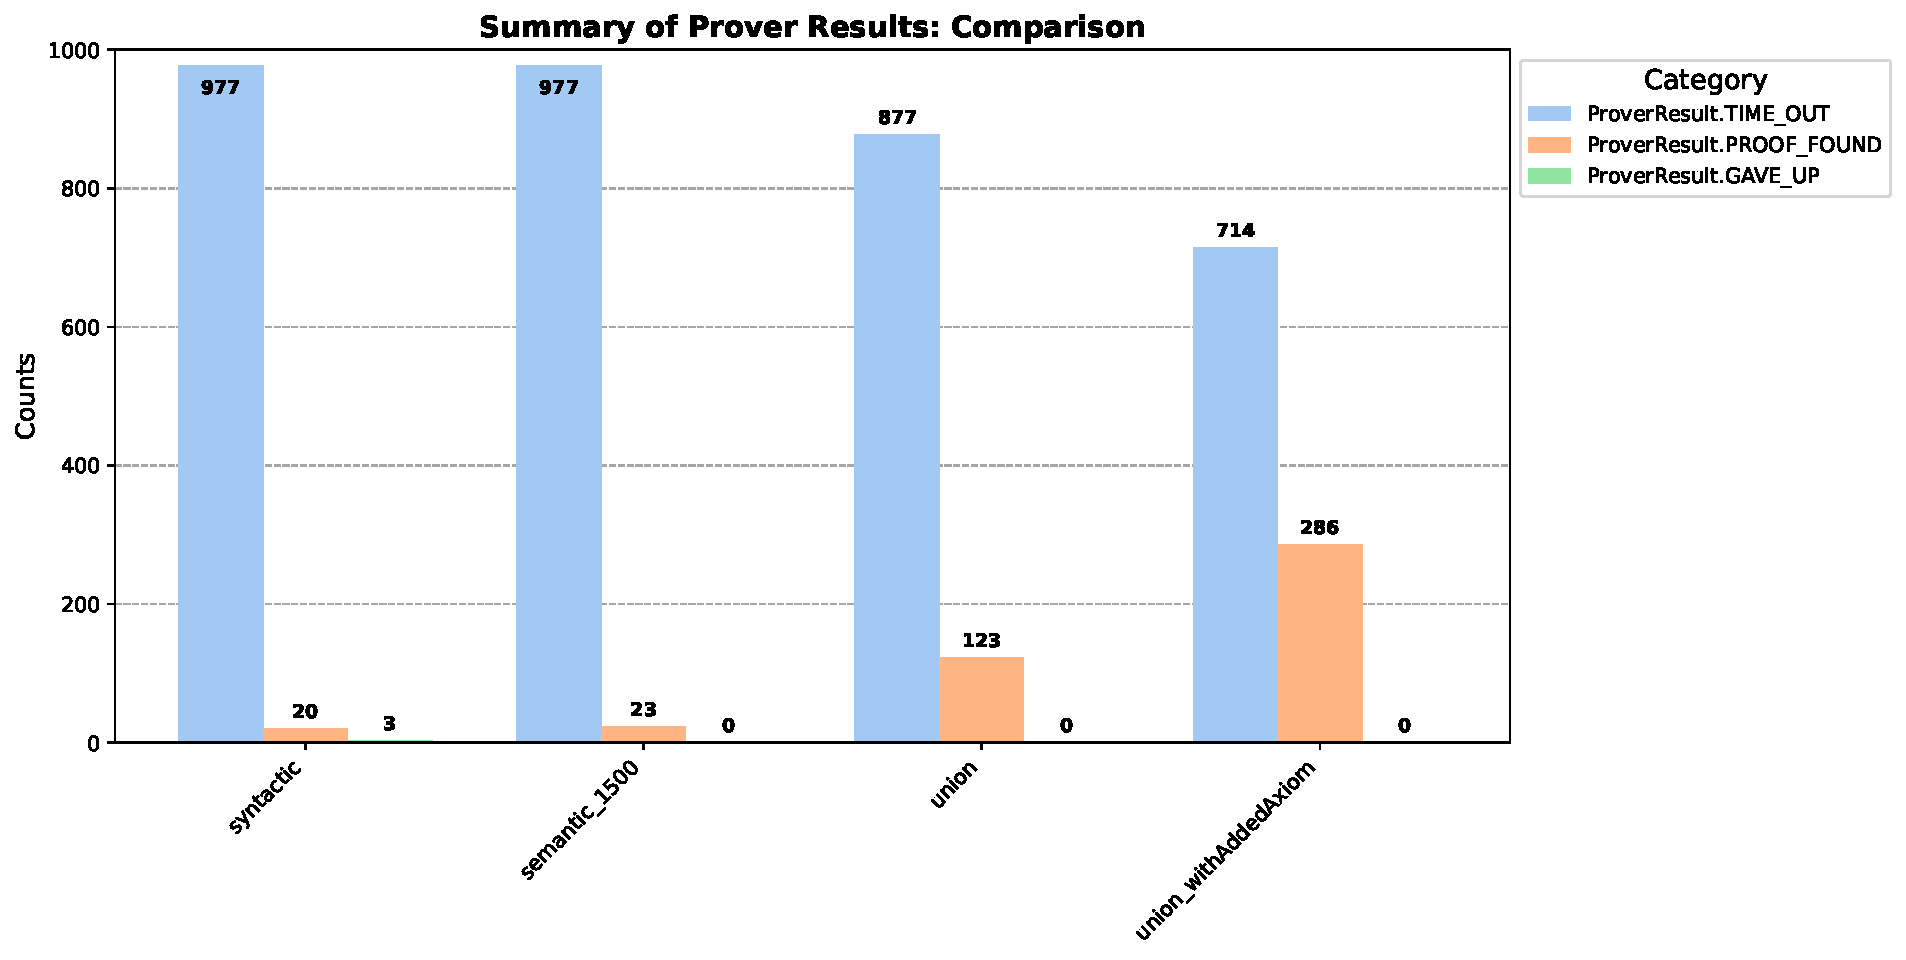
\includegraphics[width=\textwidth]{standard_mode_output.pdf} % Add path to the PDF image
      \caption{Summary of Prover Results: Standard Mode}
      \label{fig:prover_results_standard}
    \end{figure}
    \begin{figure}[h!]
      \centering
      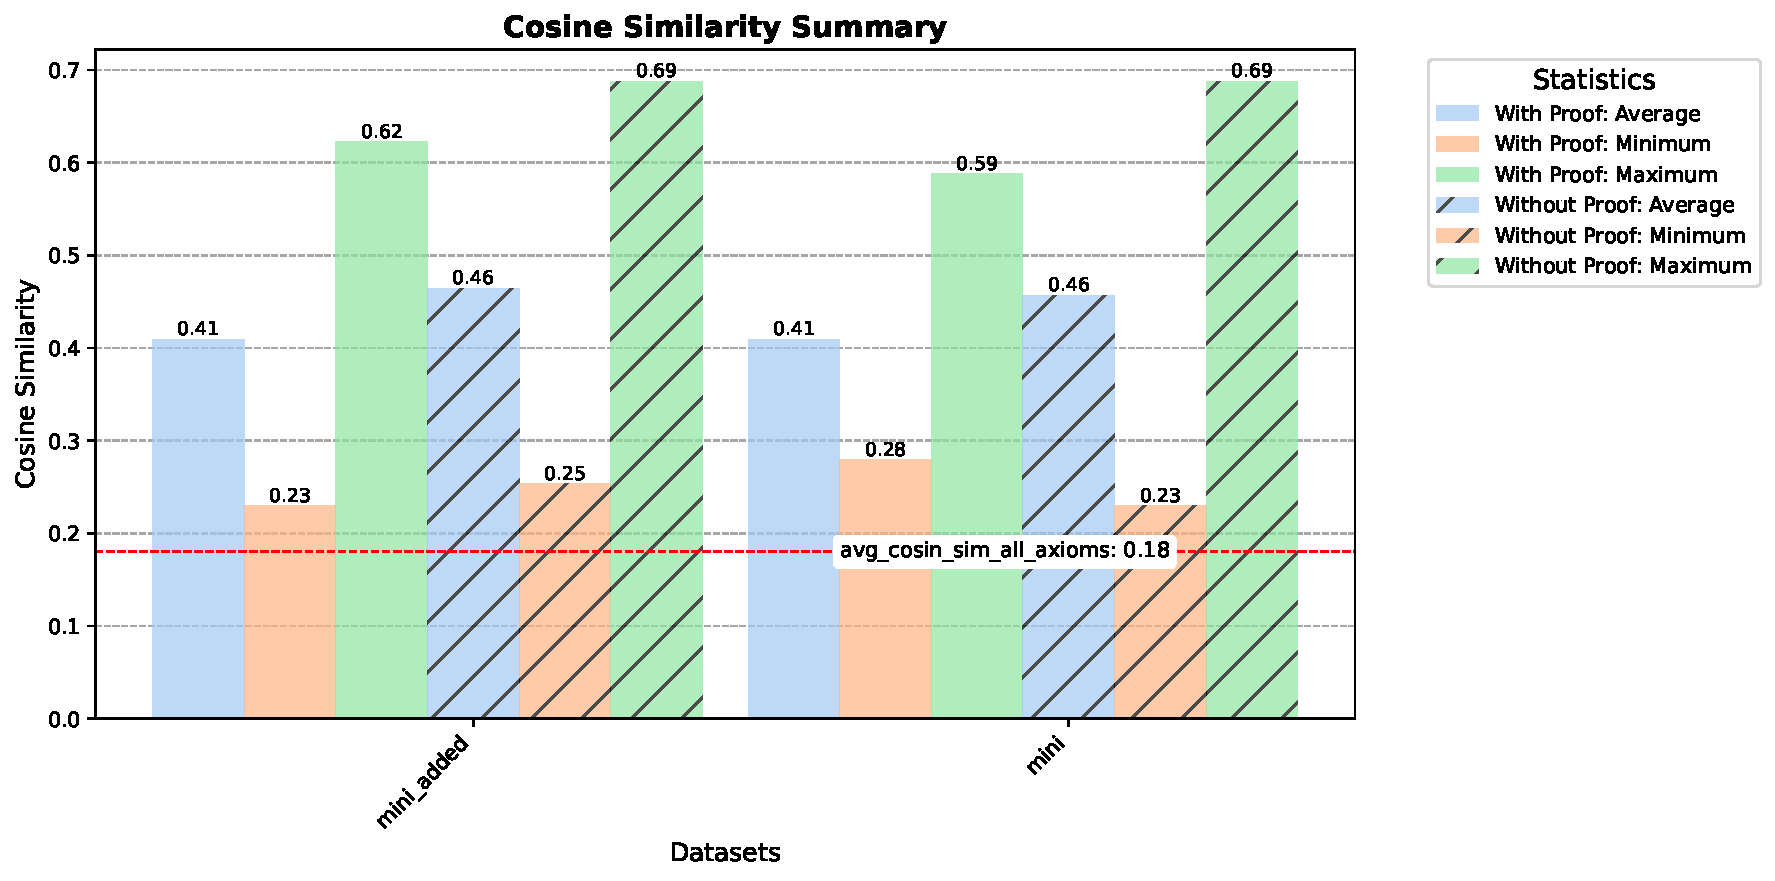
\includegraphics[width=\textwidth]{cosine_similarity_mini_summary.pdf} % Add path to the PDF image
      \caption{Summary of Prover Results: Standard Mode}
      \label{fig:prover_results_standard}
    \end{figure}
    \clearpage
    \item Modelle
    \begin{itemize}
      \item all-MiniLM-L6-v2
      \item mpnet-base-v2
    \end{itemize}
    \begin{figure}[h!]
      \centering
      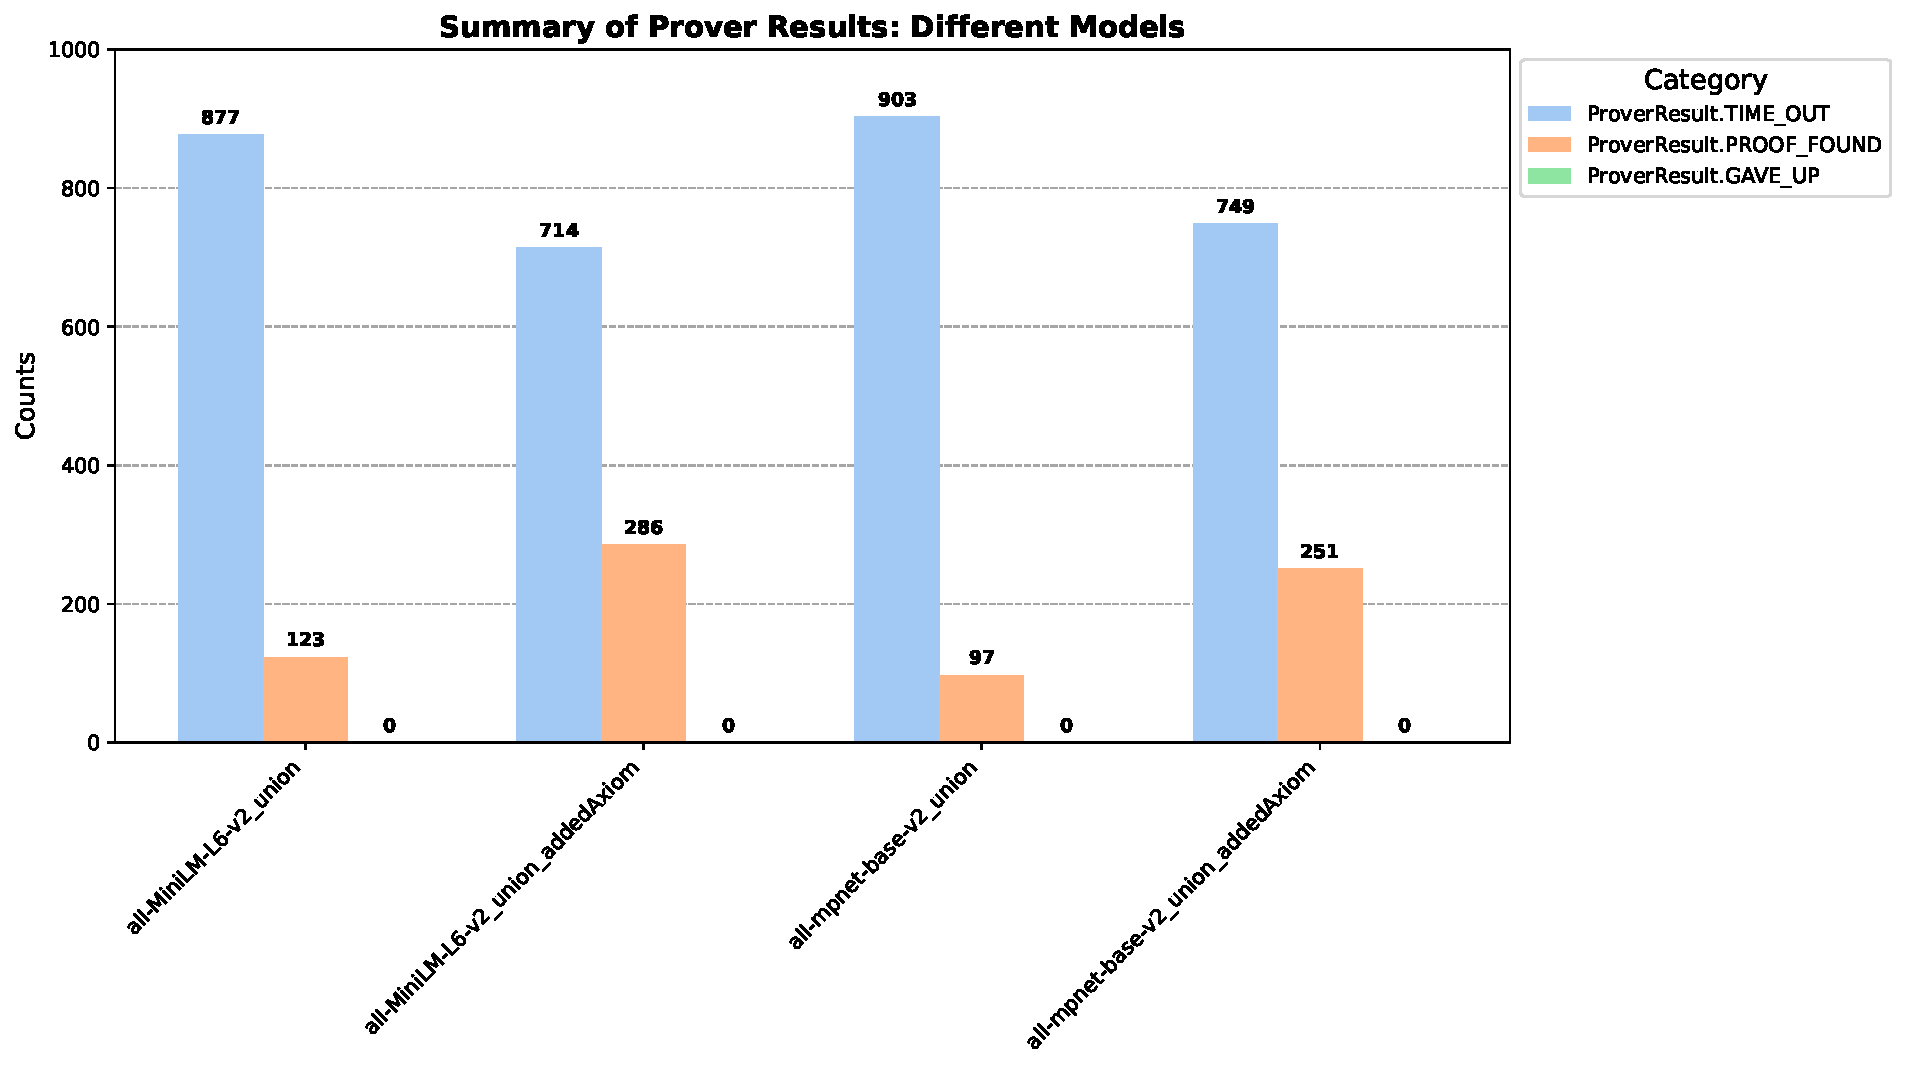
\includegraphics[width=\textwidth]{different_mode_output.pdf} % Add path to the PDF image
      \caption{Summary of Prover Results: Model Mode}
      \label{fig:prover_results_model}
    \end{figure}
    \begin{figure}[h!]
      \centering
      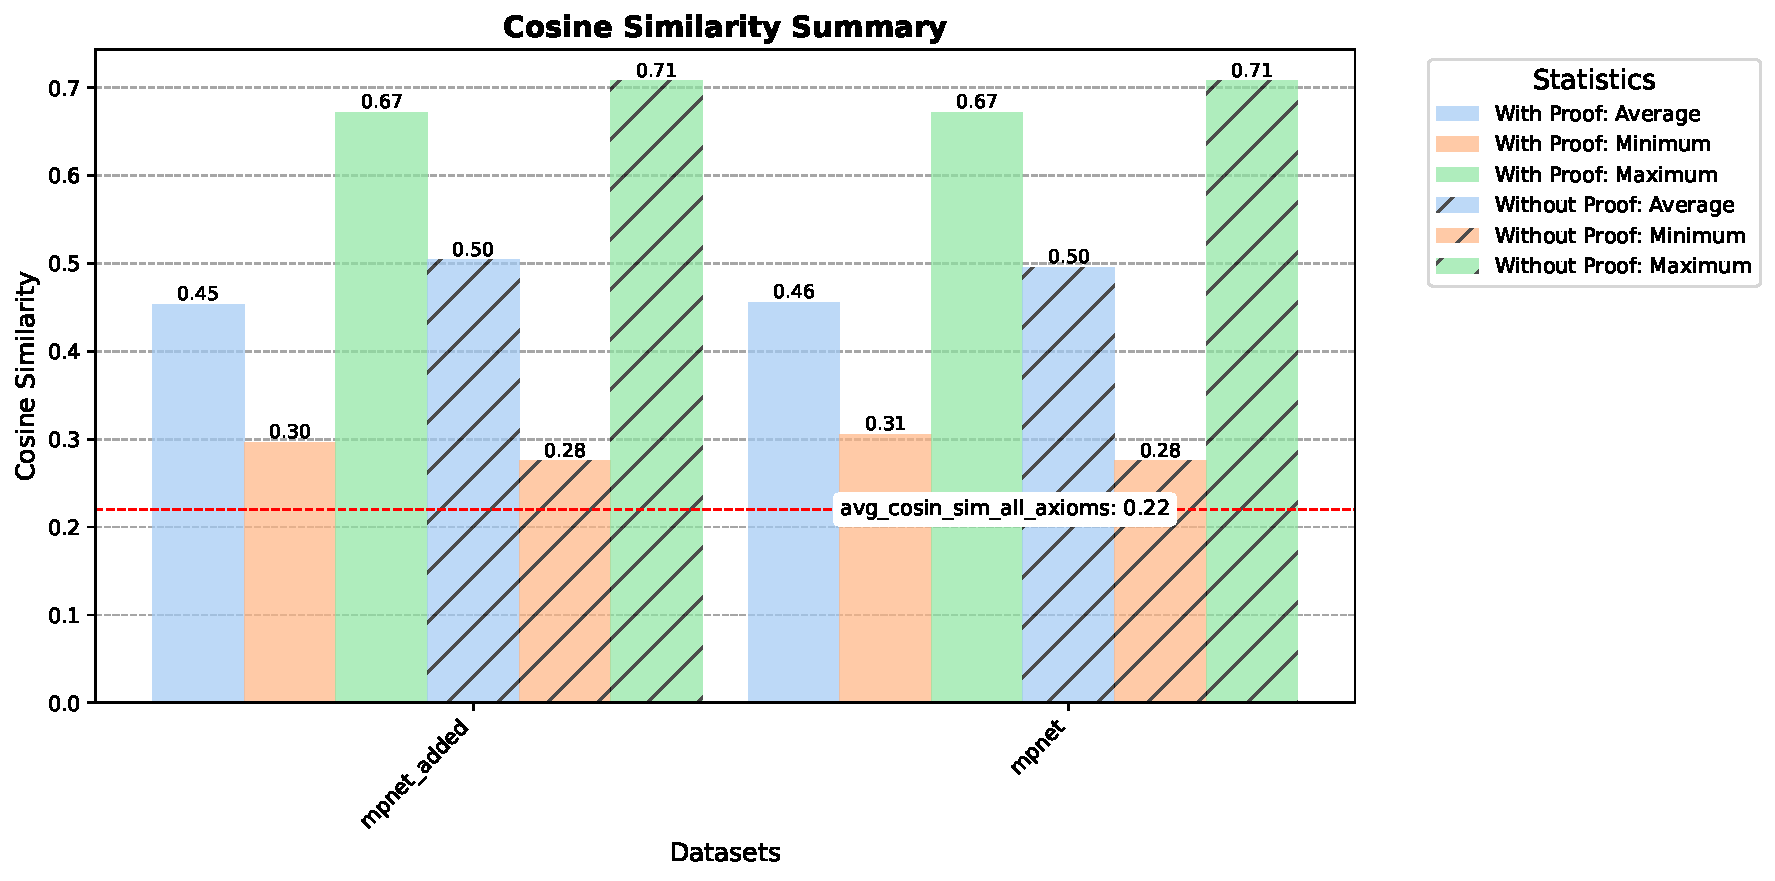
\includegraphics[width=\textwidth]{cosine_similarity_mpnet_summary.pdf} % Add path to the PDF image
      \caption{Cosine Similarity Mpnet}
      \label{fig:prover_results_model}
    \end{figure}
    \clearpage
    \item Satauto
    \begin{figure}[h!]
      \centering
      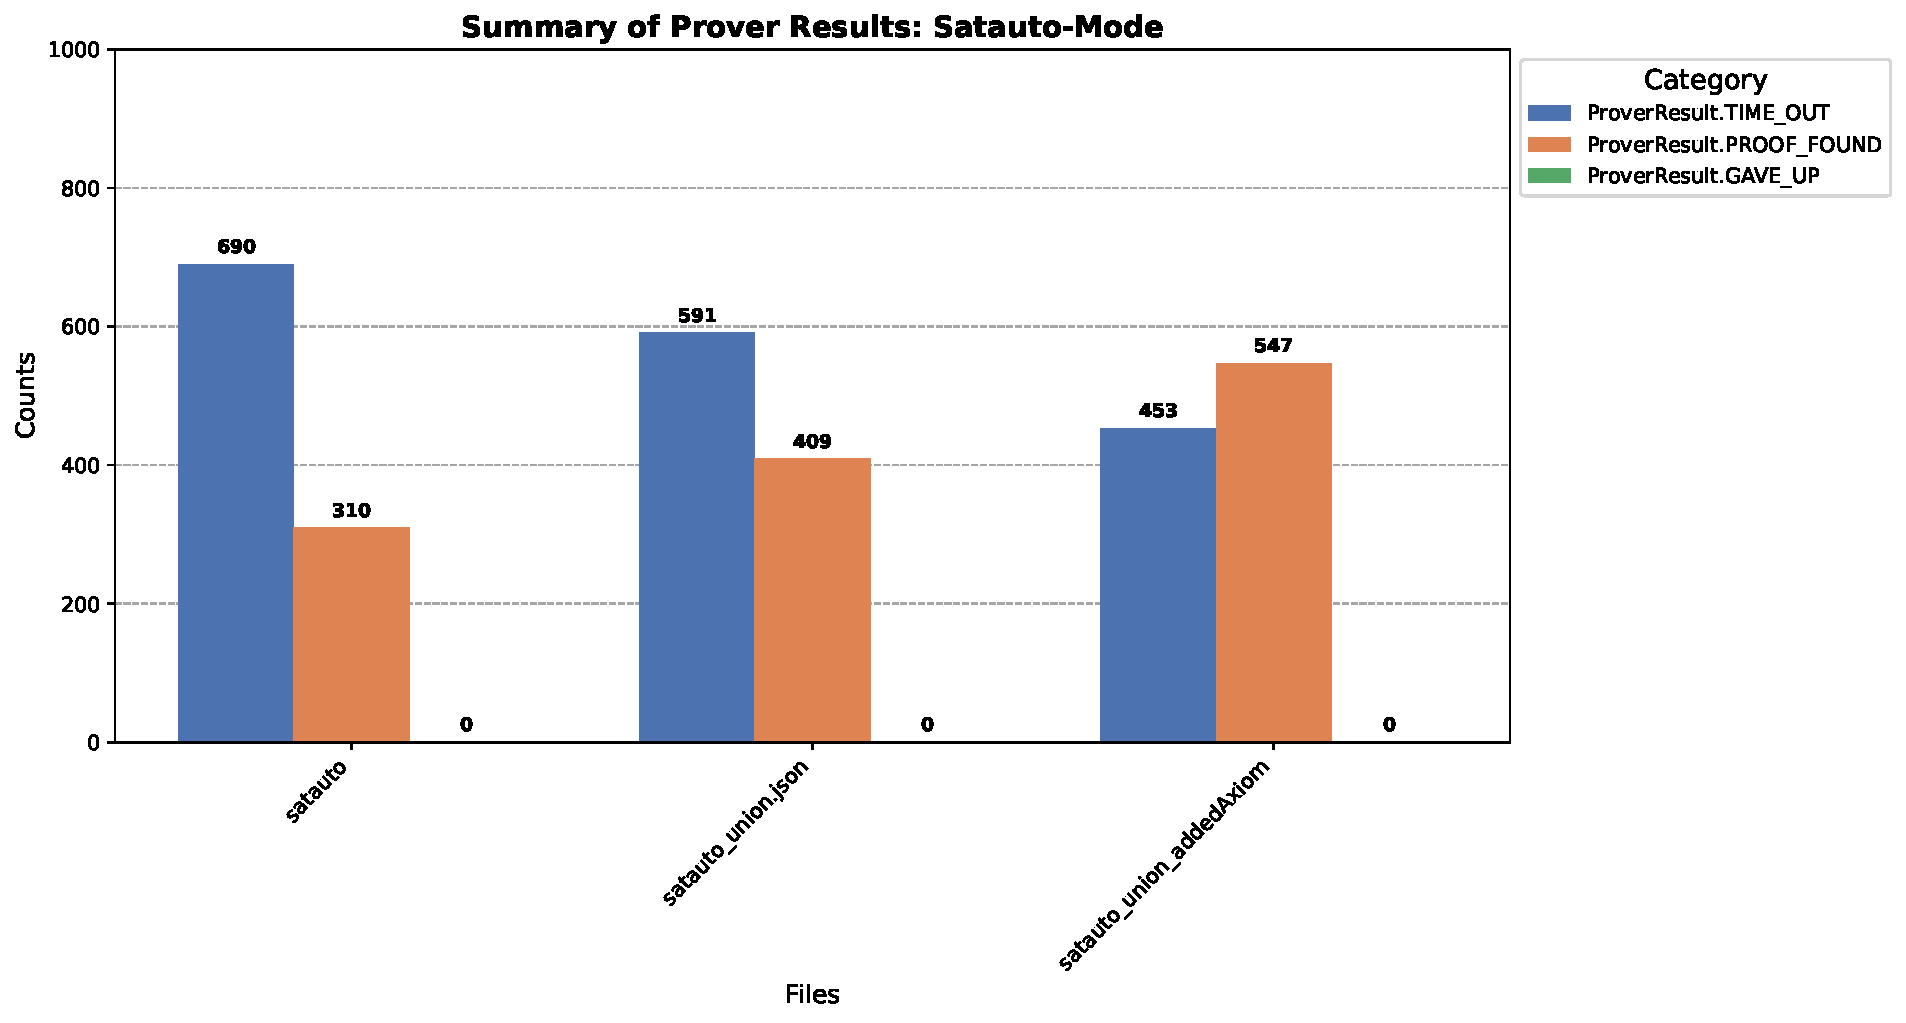
\includegraphics[width=\textwidth]{satauto_mode_output.pdf} % Add path to the PDF image
      \caption{Summary of Prover Results: Satauto Mode}
      \label{fig:prover_results_satauto}
    \end{figure}
    \clearpage
    \item Auto
    \begin{figure}[h!]
      \centering
      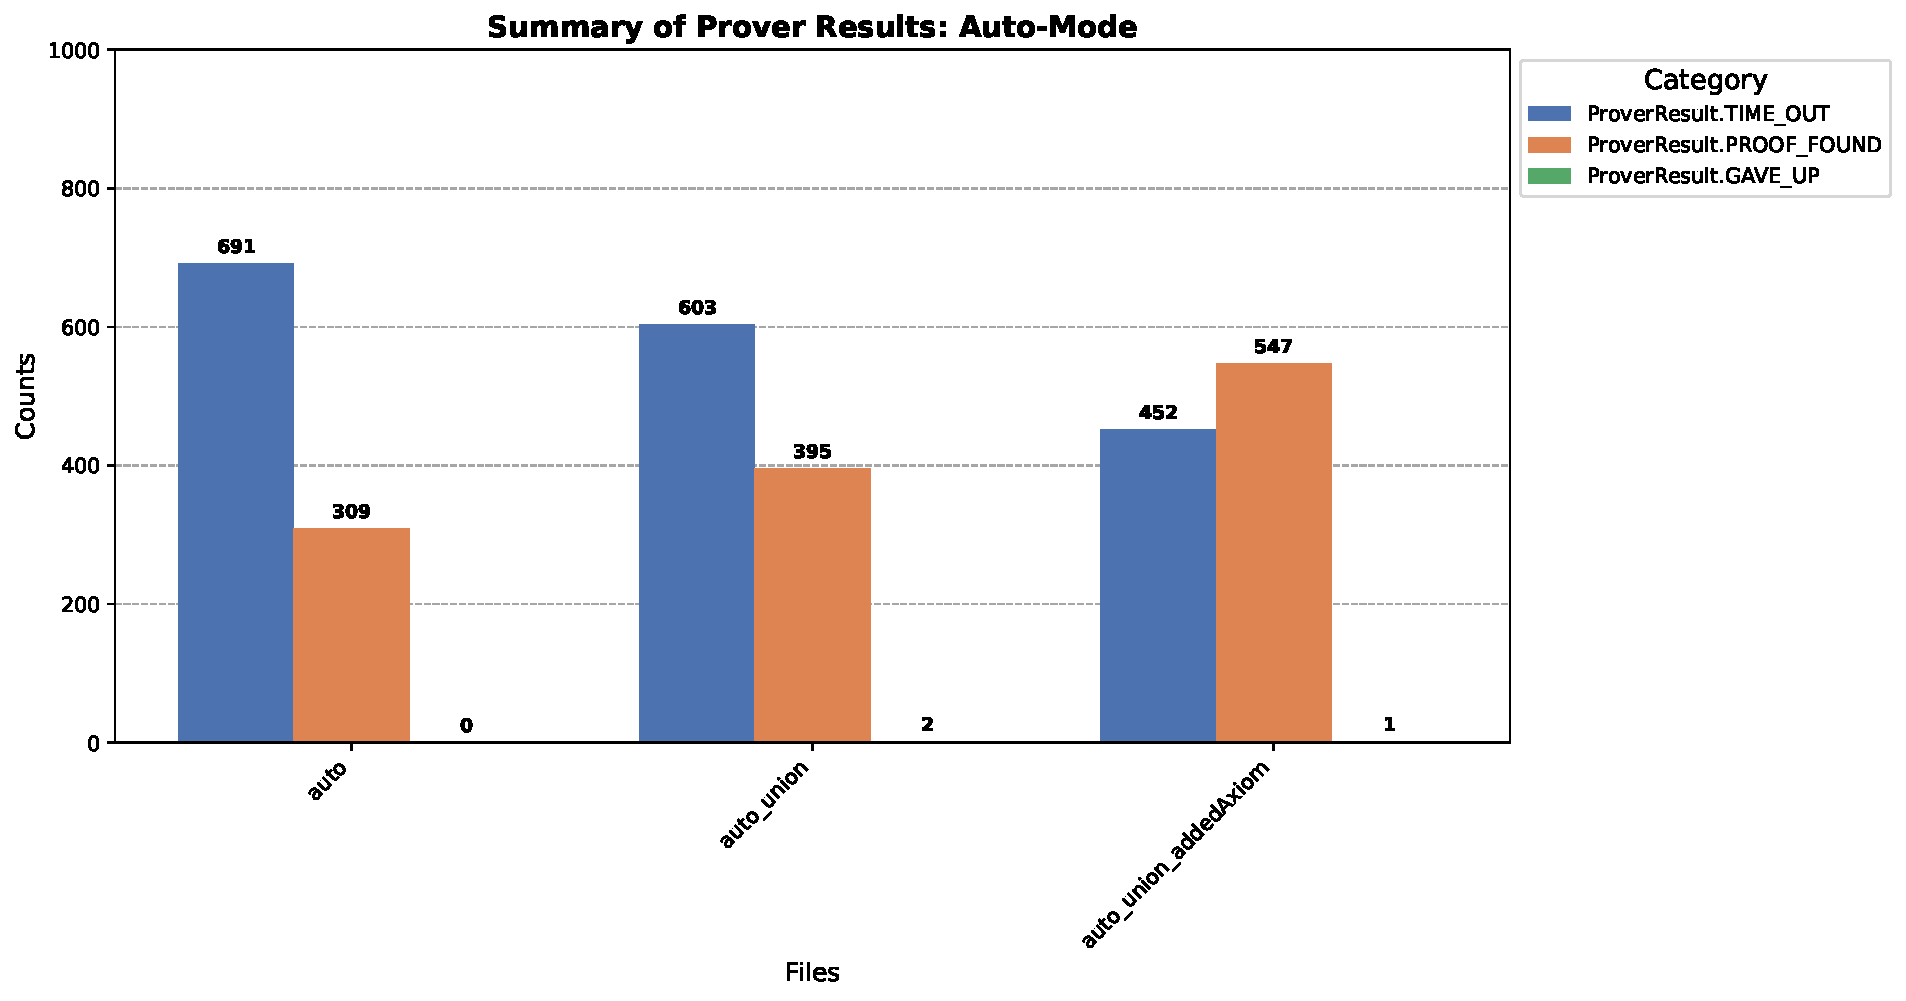
\includegraphics[width=\textwidth]{auto_mode_output.pdf} % Add path to the PDF image
      \caption{Summary of Prover Results: Auto Mode}
      \label{fig:prover_results_auto}
    \end{figure}
    \clearpage
    \item Vampire
    \begin{figure}[h!]
      \centering
      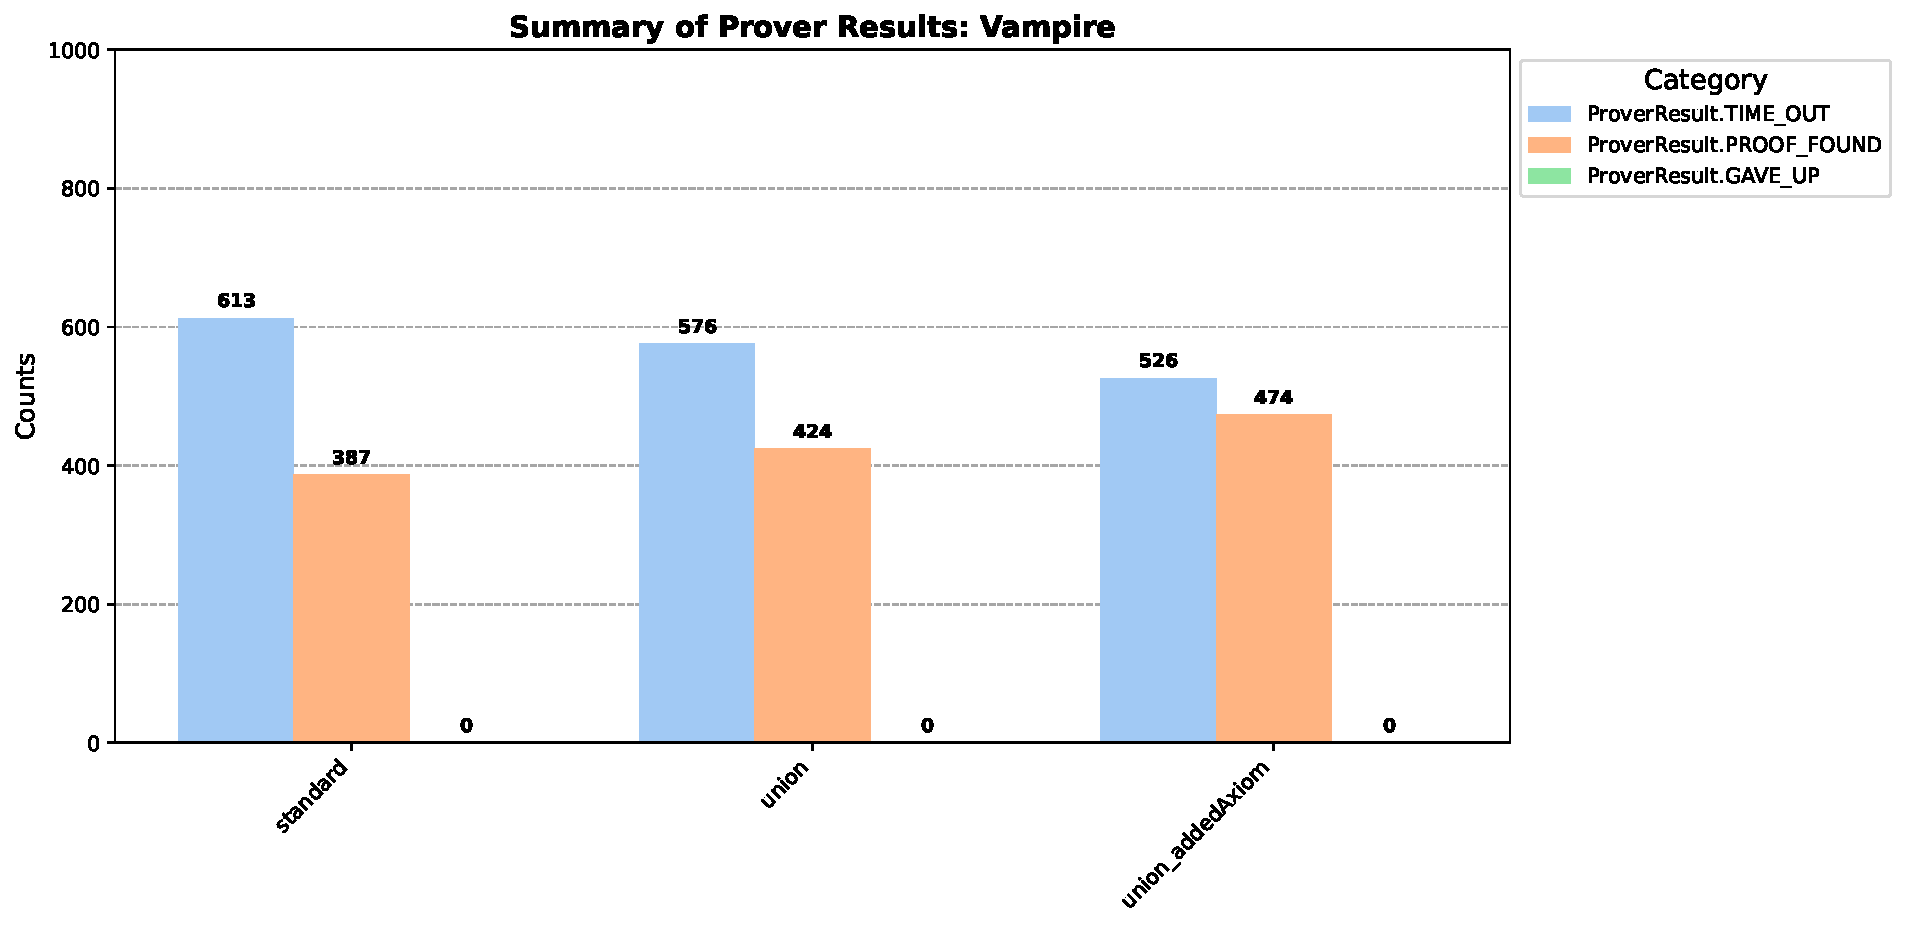
\includegraphics[width=\textwidth]{vampire_mode_output.pdf} % Add path to the PDF image
      \caption{Summary of Prover Results: Vampire Mode}
      \label{fig:prover_results_vampire}
    \end{figure}
    \clearpage
    \item Statistiken
      \begin{itemize}
        \item Proofs found in first named
        \begin{figure}[h!]
          \centering
          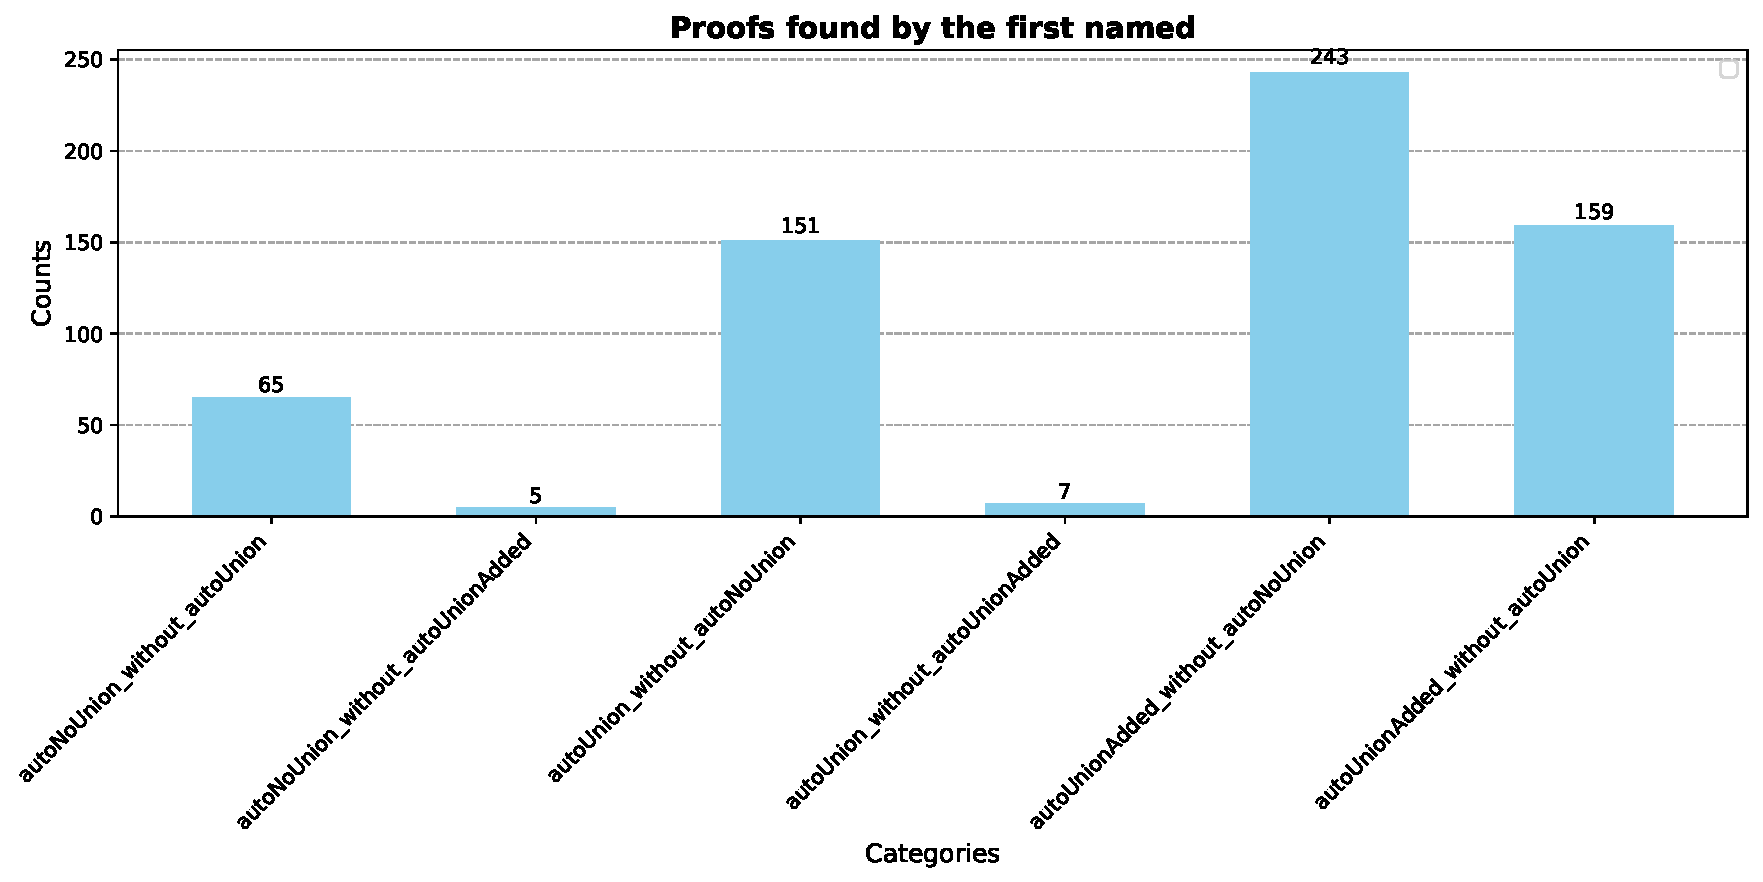
\includegraphics[width=\textwidth]{proof_found_difference.pdf} % Add path to the PDF image
          \caption{Summary of Prover Results: Proofs found}
          \label{fig:prover_results_proof_found}
        \end{figure}
        \clearpage
        \item Time to find proof
        \begin{figure}[h!]
          \centering
          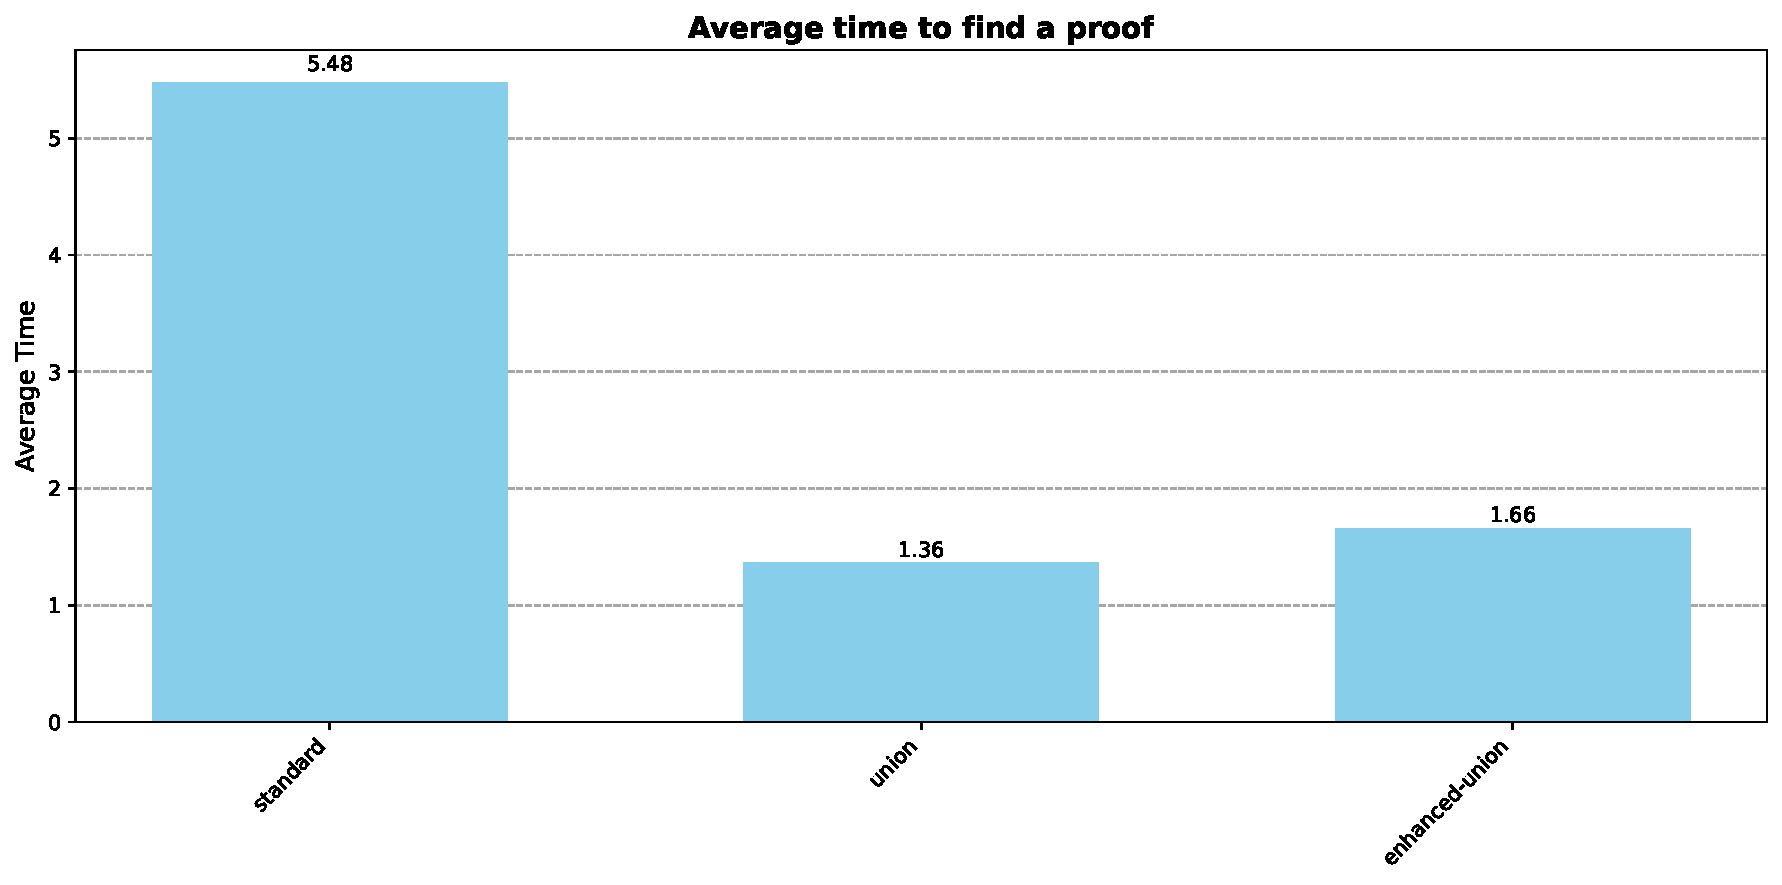
\includegraphics[width=\textwidth]{time_to_find_proof.pdf} % Add path to the PDF image
          \caption{Summary of Prover Results: Proofs found time}
          \label{fig:prover_results_proof_found}
        \end{figure}
        \clearpage
        \item Time to find common proof
        \begin{figure}[h!]
          \centering
          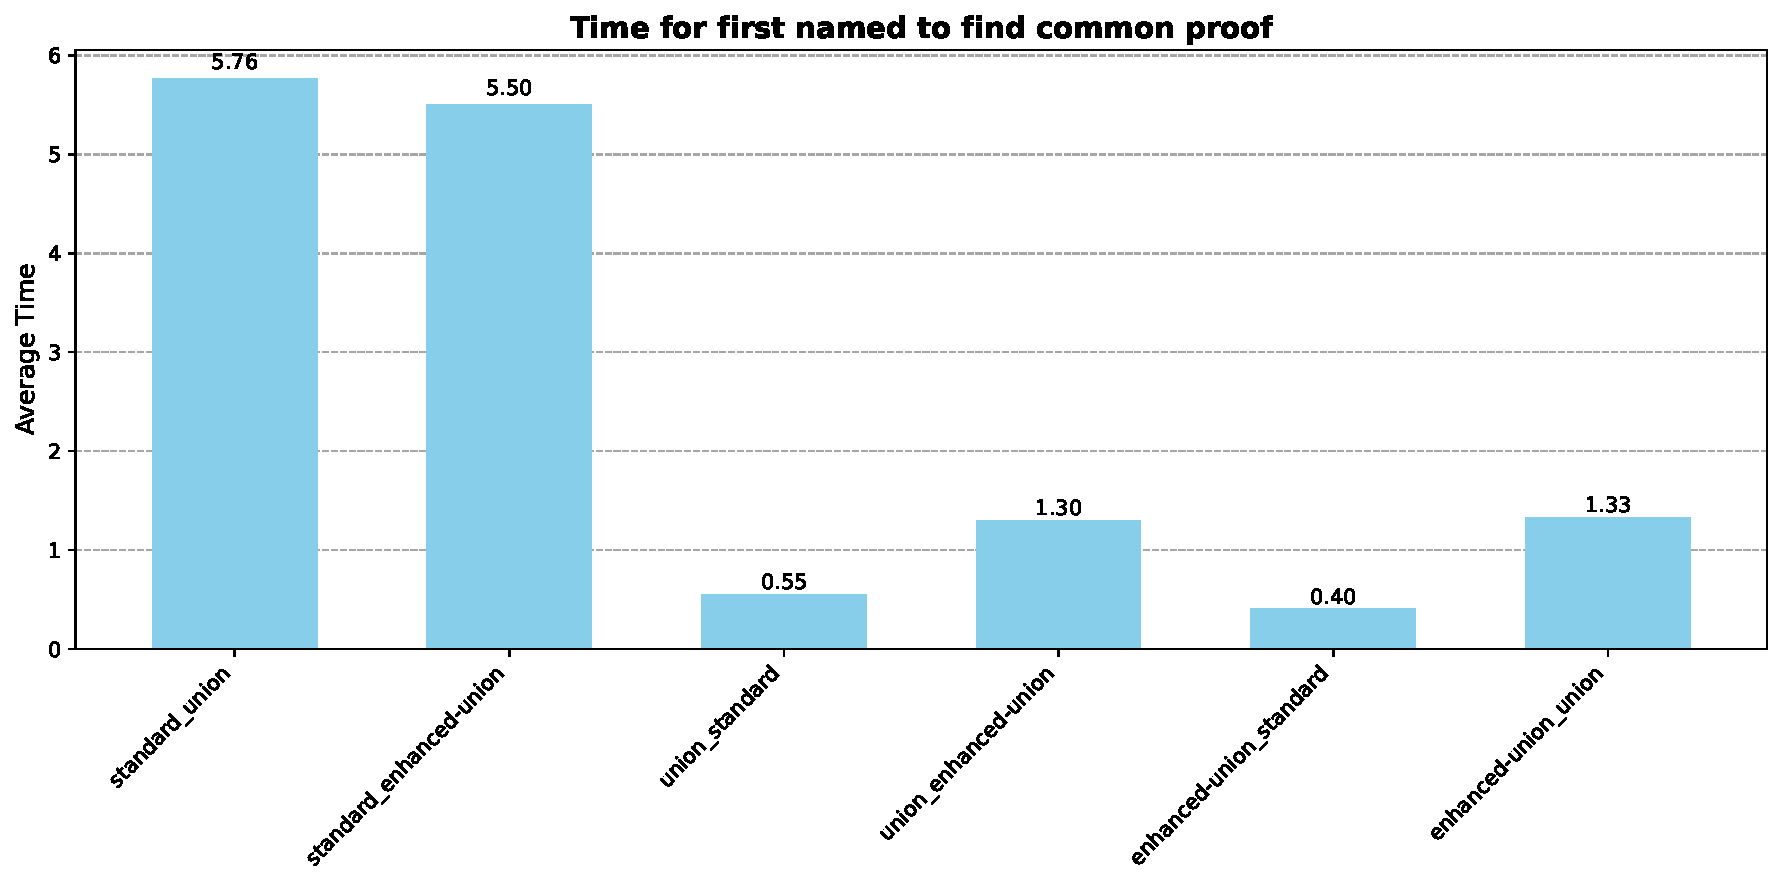
\includegraphics[width=\textwidth]{time_to_find_common_proof.pdf} % Add path to the PDF image
          \caption{Summary of Prover Results: Common proofs found time}
          \label{fig:prover_results_proof_found}
        \end{figure}
        \clearpage
      \end{itemize}
    \item Conclusion
  \end{itemize}
\chapter{Weiterführende Arbeit}
\begin{itemize}
  \item Wahl der richtigen Axiome durch neuronales Netz
\end{itemize}
\chapter{Quellenverzeichnis}
\end{document}